\newpage
\section{人体二维姿态估计问题的研究}
\subsection{问题描述}
在计算机视觉领域中,人体二维姿态估计是一个极具挑战的任务,人体二维人体姿态估计问题,即是说给定输入的图片或视频序列,进行处理得到相应的人体各个关节在图片上的位置。在深度学习普及之前,该领域的主要研究方法是基于传统的图像处理方法,从图片中提取特征然后进行检测,但是这些传统的处理方法准确率与精度都较低,难以推广到一般场景。自从深度学习方法开始普及之后,对于二维人体姿态估计问题,由于可以由人类标注者在图像中标出人体的关节点的位置,因此可以得到大量的这样的带标注的的训练数据。而基于深度神经网络的方法就可以利用这样大量的数据,对网络进行训练。因此目前的主流的准确率较高的方法都是基于深度学习技术的,本文因此也只介绍这部分内容。如图\ref{fig:2dimage}为我们采集的三个不同的演员的图片示例,图中的数据采集时间为2019年4月28日,文中使用的分别对应于原数据中演员冯的第9个相机的第15帧,演员帅的第5个相机的第990帧,演员柯的第1个相机的1604个相机。由于采集得到的数据量较大,因此在文中无法一一展示,因此我们只选择了部分图片作为样例说明。二维姿态估计任务就是从这样的图片中去获取人体的关节点在图中的位置。

\begin{figure}[htbp]
    \centering
    \subfigure[演员冯]{
        \begin{minipage}[t]{0.3\linewidth}
            \centering
            \includegraphics[width=\linewidth]{figure/result/images/feng2} %
        \end{minipage}% 
    }% 
    \subfigure[演员帅]{
        \begin{minipage}[t]{0.3\linewidth}
            \centering
            \includegraphics[width=\linewidth]{figure/result/images/shuai2} %
        \end{minipage}% 
    }%
    \subfigure[演员柯]{
        \begin{minipage}[t]{0.3\linewidth}
            \centering
            \includegraphics[width=\linewidth]{figure/result/images/ke2} %
        \end{minipage}% 
    }%  
    \caption{LightStage数据采集样例\label{fig:2dimage}}
\end{figure}

\subsection{研究方法比较}
人体二维姿态估计目前有两个主流方案,第一种是自顶向下的方法,这种方法先检测图片中的人体,得到一个人体的检测框,然后去分别检测每一个人的人体区域中的姿态;另一种是自底向上的方法,首先检测出图片中的所有的人的肢体的关节节点,然后将关节节点进行拼接,得到人体的骨架。自顶向下的方法中,姿态检测的准确度会依赖于人体区域框的检测质量,如果人体区域框的检测不够稳定,那么该方法的输出也会相应的变差。并且如果图片中的人数增加,那么该算法检测到的人体区域的框就会增加,同样的计算时间也会成倍地增加。但是对于自底向上的方法来说,由于是对整张图进行检测,因此计算时间不会随着图片中人数的增加而成倍增加,同时也不会受到前一步检测的人体区域框的质量的影响,检测结果更加鲁棒。但是在自底向上的方法中,如果两个人离得较近,会出现拼接错误的情况;同时由于这种方法依赖的是关节之间的联系,所以对全局信息的获取会有不足。

目前主流的开源人体二维检测方案主要有几种,并且在不同的场景中各有优劣。为了在我们的数据上取得较好的效果,我们对三种方法都进行了研究,并进行了测试,以下依次介绍三种模型。

\subsubsection{OpenPose}
OpenPose\cite{openpose}是由卡耐基梅隆大学的Gines Hidlalgo等人提出的多人二维关键点实时检测方案,该方案是第一个实时的多人二维关键点检测系统,能够同时检测认的身体关键点、手部关键点、脸部关键点及脚部关键点(总共135个关键点)。该方案是基于自底向上的思想的。该方法使用了一种叫部件亲和场(Part Affinity Fields,简称PAF)的非参数表示方法,通过这种方法将检测出来的人体关节组合起来。部件亲和场的表示方法是指,对于人体上的骨架上的每一个像素,去回归这一段骨架的方向向量。如图\ref{fig:2d-op}-(c)所示,对于输入的图片中人体的手臂部分,OpenPose会去回归一个这个手臂上的点沿着人体的关节顺序的指向的方向。例如对于手臂一段,手肘与手腕中间的属于人体的部分的像素,就会输出一个向量表示方向,这些向量都会从手肘指向手腕。该方法具有较高的精度以及较好的实时性。该方法可以同时对人体的身体部分、双脚、手部关节点、脸部关键点进行检测,输出结果较为丰富。
\begin{figure}[H]
    \centering
    \includegraphics[width=\linewidth]{figure/2dpose/openpose}
    \caption{\label{fig:2d-op} OpenPose流程图}
\end{figure}
该方法主要分为几个步骤,其流程图如图\ref{fig:2d-op}所示。首先对于一张输入的尺寸为\(w\times h\)的图片,如图\ref{fig:2d-op}-a,OpenPose将整张图片输入给前馈神经网络,通过该网络预测一系列的二维位置置信图(confidence map)\(\mathbf{S}\),置信图表示的人人体的关节的位置,如图\ref{fig:2d-op}-b所示,以及一系列的二维关节亲和向量场(PAFs)\(\mathbf{L}\),如图\ref{fig:2d-op}-c所示。对于一个人体,如果有\(J\)个关节,那么这一步就会输出\(J\)张置信图,即\(\mathbf{S}=(\mathbf{S}_1, \mathbf{S}_2, ..., \mathbf{S}_J)\)每一张代表了人体的一个关节,其中\(\mathbf{S}_{j}\in \mathbb{R}^{w\times h}$, $j \in \{1\ldots J\}\)。输出的部件亲和场总共有\(C\)个,每一个代表了定义的人体的每一段骨头,即\(\mathbf{L}_{c}\in \mathbb{R}^{w\times h \times 2}$, $c \in \{1\ldots C\}\),其中对于每一段骨头的部件亲和场表示的是一个二维的向量场,\(\mathbf{L}_{c}\in \mathbb{R}^{w\times h \times 2}, c \in \{1\ldots C\}\)。最后通过对回归的结果进行组合,使用贪心策略匹配属于同一个人的关节,就能得到整个人体的完整的身体姿态。如图\ref{fig:2d-op}-e所示。

\begin{figure}[H]
    \centering
    \includegraphics[width=\linewidth]{figure/2dpose/openpose-arch}
    \caption{\label{fig:2d-op-net} OpenPose网络结构}
\end{figure}
OpenPose的网络结构如图\ref{fig:2d-op-net}所示。该网络是一个多阶段的卷积神经网络,图中的蓝色部分负责预测部件亲和场,橙色部分负责预测置信图。由于网络是多阶段的,因此上述两个模块可以不断堆叠在一起,并且对每一个阶段都进行监督,相当于对检测结果不断进行优化。网络中的每个卷积模块使用的是三个堆叠在一起的卷积核为\(3\times 3\)的卷积网络。在输出置信图和部件亲和场后需要对不同的人的身体关节进行组合,由于本文研究的场景都是单人的,因此该部分暂时先不考虑。

\subsubsection{AlphaPose}
AlphaPose\cite{AlphaPose}是上海交通大学卢策吾教授团队开源的二维人体关键点检测方法,该方法使用的是自顶向下的方法,即首先检测人体所在的框的区域,再对框中的人体进行关键点检测。
\begin{figure}[H]
    \centering
    \includegraphics[width=\linewidth]{figure/2dpose/alphapose}
    \caption{\label{fig:2d-ap} AlpahPose流程图}
\end{figure}
该算法流程图如图\ref{fig:2d-ap}所示。首先通过区域候选网络(Region Proposal Network,简写为RPN)提出候选的人体区域,然后将所得到的所有的候选的人体区域框分为两支。图中\ref{fig:2d-ap}上一支通过了空间变换网络(Spatial Transformer Network,简写为STN),将不规则形状的框转化到统一的空间内进行单人的人体姿态估计(Sigle-Person Pose Estimator,简写为SPPE),再将结果通过空间反变换网络(Spatial Detransformer Network,简写为SDTN)转化到原始图片坐标系中。另一支直接通过单人姿态估计(Single Person Pose Estimation)算法,进行姿态估计。最后将两支的结果融合,通过姿态非极大值抑制算法得到姿态。

\subsubsection{级联金字塔网络}
级联金字塔网络(Cascaded Pyramid Network, 简称CPN)\cite{CPN}是由旷视科技提出的模型,该模型取得了COCO2017人体关键点挑战赛的冠军,该模型主要面向的问题是单张图片中的多人姿态估计问题。该模型属于自顶向下的方法,即也是首先生成人体的边界框,之后对单个人体的框进行关键点检测。
\begin{figure}[H]
    \centering
    \includegraphics[width=\linewidth]{figure/2dpose/cpn}
    \caption{\label{fig:2d-cpn} CPN流程图}
\end{figure}
该网络的流程图如图\ref{fig:2d-cpn}所示。级联金字塔网络包含了两个阶段,第一个阶段为全局网络(GlobalNet),这部分用来从图像中提取特征,可以定位特征较为明显的关键点,例如手和脚,但是无法直接从图片中识别出被遮挡的关键点;第二个阶段为精炼网络(RefineNet),这一阶段主要通过整合全局网络中识别得到的图片特征,来推断被遮挡住的关键点的位置。即是说理解可以看到的关键点所提供的上下文信息,完成所有关键点的检测任务。

论文中的全局网络的骨架是深度残差网络\cite{resnet},通过使用U形结构来整合不通尺度的空间分辨率的特征以及语义信息。精炼网络部分中,为了提高计算的效率,同时保持信息在传输过程中的完整性,精炼网络部分首先讲不同尺度的特征图进行堆叠,然后通过上采样和融合,将不同层次的信息进行融合。

\subsection{模型比较}
为了验证上述二维关节点检测模型在我们的实验环境下的准确度,我们需要对其进行定量的分析。
\subsubsection{数据集介绍}
由于我们的实验设备没有在人身上贴标签,因此无法得到准确的三维关键点以及二维关节点的坐标,因此我们选择了广泛使用的Human3.6M数据集\cite{ionescu2014human3}。该数据集是最大的人体三维姿态数据集之一,包含了360万的图片,其中包括了11个演员以及15个日常动作,例如吃饭,走路等。该数据集的采集环境为室内环境,并且使用了总共4个相机来进行数据采集。该数据集通过在人体贴上标志物来获得人体的三维空间的关节位置,相对于从图片直接估计来说较为准确,因此我们通过该数据集来对我们的算法进行定量分析。

\subsubsection{评价标准}
由于我们的任务是进行单人的二维关键点检测,因此不需要考虑多人的二维关键点评价标准。而由这些模型公开的评价指标的数值均是针对多人场景的,因此我们需要对自己得到的结果进行测量。在这里,我们直接使用了在图像中的像素误差值作为真实值与估计值计算的距离,使用的评价标准为平均关节误差,计算公式为
\begin{equation}
    e = \frac{\delta(v_i)\sum_i d_i}{\sum_i\delta(v_i)}
\end{equation}
其中\(d_i\)表示测量的该关节的位置与真实的关节位置的欧式距离,一般写为\(d_i = \sqrt{(\hat{x_i} - x_i)^2 + (\hat{y_i} - y_i)^2}\),这里的\(v_i\)表示第\(i\)个关节的可见性,如果这个关节在图中可见,那么\(v_i = 1, \delta(v_i) = 1\),反之,如果该关节不可见,那么\(v_i = 0, \delta(v_i) = 0\)。这里使用\(\delta\)函数是因为一般的模型输出的是一个介于0-1之间的值,表示其可见性的不确定度。
% 在进行人体二维关键点任务的评价时,一般使用的指标是\textbf{关键点相似度}(Object Keypoint Similarity,简称OKS)。因为对于人体来说,如果简单的使用欧氏距离来进行计算的话,相当于没有考虑到人体在图像中的大小会随着距离的改变而改变。因此该指标会考虑到人体的尺度,计算公式为:
% \begin{equation}
%     OKS_p = \frac{\sum_i }{-d^2_}
% \end{equation}

在这一部分中,我们使用Human3.6M数据集的图片,通过三种不同的人体二维关节点检测方法获得其关节位置,与其提供的二维关节点的位置进行比较,计算三种方法的误差。由于二维关节点的训练数据集中,关节的位置通常都是由人类标注者进行标注,而Human3.6M的关节点的位置是由其贴的标志的位置决定的,因此两者的关节定义有所不同,而在三种二维关节点检测方法中,其各自使用的训练数据集也有所区别,因此我们只选择了人的身体上的主要的几个点进行比较。
\begin{figure}[htbp]
    \centering
    \subfigure[原始图片]{
        \begin{minipage}[t]{0.23\linewidth}
            \centering
            \includegraphics[width=\linewidth]{figure/2dpose/h36m} %
        \end{minipage}% 
    }% 
    \subfigure[OpenPose结果]{
        \begin{minipage}[t]{0.23\linewidth}
            \centering
            \includegraphics[width=\linewidth]{figure/2dpose/h36mop} %
        \end{minipage}% 
    }%
    \subfigure[CPN结果]{
        \begin{minipage}[t]{0.23\linewidth}
            \centering
            \includegraphics[width=\linewidth]{figure/2dpose/h36mcp} %
        \end{minipage}% 
    }%  
    \subfigure[AlphaPose结果]{
        \begin{minipage}[t]{0.23\linewidth}
            \centering
            \includegraphics[width=\linewidth]{figure/2dpose/h36map} %
        \end{minipage}% 
    }%   
    \caption{三种人体二维检测框架在Human3.6M \cite{ionescu2014human}上的结果示例\label{fig:h36mres}}
\end{figure}

\subsubsection{测试结果}
我们取了Human3.6M数据集中的一段视频,该段视频包含了5783帧,时长为1分57秒,视频帧率为50帧每秒。每一个相机拍摄的图片的分辨率为\(1000\times 1002\),与我们的图片的分辨率接近。每一帧有四个视角的相机,即总共有23132张图片,我们对所有的图片都测试了一遍三种模型,得到其各自的结果,运行环境为CPU为 Intel i7-8700,8G RAM,显卡为GeForce GTX 1060 6GB GPU,系统平台为Ubuntu 16.04。OpenPose的源代码为C++实现,需要对源代码进行编译,得到可执行文件运行;AlphaPose基于PyTorch实现,需要配置PyTorch 1.0版本的环境;CPN是基于TensorFlow实现的代码,配置TensorFlow 1.9.0版本即可运行代码。代码配置过程此处省略不表。

三种模型的二维关键点检测结果如图\ref{fig:h36mres}所示。从可视化的结果来看,三种模型的检测结果基本一致,我们需要进一步的定量计算。在这里计算时,由于网络输出具有不确定性,对每个关节的结果都会由一个范围为\((0,1)\)的置信度,我们这里进行量化的时候只考虑那些置信度大于0.5的关节检测结果。首先计算三种方法的检测的平均关节误差,如表\ref{tab:2derror}所示。从表\ref{tab:2derror}中可以看出,AlphaPose的误差均值最低,并且数据的离散程度也较低。OpenPose方法虽然在多人的场景下表现较好,但是在这种单人背景简单的场景下表现不如自顶向下的两种方法。
\begin{table}[H]
    \centering
    \begin{tabular}{lccc}
        \hline
        Name                    & OpenPose & CPN     & AlphaPose \\
        \hline
        \text{误差均值(像素)} & 9.62  & 9.32 & 8.78   \\
        \text{误差标准差}       & 6.35  & 7.85 & 4.63   \\
        \hline
    \end{tabular}
    \caption{三种二维检测人体方法的误差\label{tab:2derror}}
\end{table}

为了更直观的观察其误差,我分别计算了各个关节的误差的分布,并统计了各个关节误差的直方图,如图\ref{fig:2d-loss}所示。从表\ref{tab:2derrorjoint}中可以看出,对于接近人的躯干的部位,如臀部和肩部,其误差的波动大多比处于人的躯干末端的部位小。从误差的直方图中可以看出,对于躯干上的关节点(躯干只左右肩、左右臀部),其误差分布比较接近正态分布,数据都集中在一块,且极差相对较小。而对于属于手和脚的关节点,如图\ref{fig:2d-loss}的第二、三列所示,会出现极个别的误差特别大的点。经过可视化发现,这些误差大的地方主要是人的左右出现了误匹配的情况,因此其置信度较大,但是实际上是匹配错误的,这也是深度神经网络的缺陷之一。因此我们需要在接下来的工作中考虑如何去除掉这些误匹配的离群点,如何利用多视图的信息来对离群点进行剔除。
\begin{table}[H]
    \centering
    \begin{tabular}{lcccccc}
        \hline
        名称      & 左臀     & 左膝    & 左踝     & 右臀     & 右膝    & 右踝     \\
        \hline
        OpenPose  & 11.5,6.0 & 8.8,6.4 & 15.9,7.6 & 15.9,5.0 & 8.0,7.4 & 11.1,9.8 \\
        CPN       & 11.4,5.9 & 7.7,5.5 & 14.0,7.8 & 16.2,5.1 & 6.9,6.6 & 9.8,8.2  \\
        AlphaPose & 12.2,5.2 & 7.8,4.3 & 13.6,5.7 & 17.2,5.2 & 6.7,5.0 & 9.6,5.6  \\
        \hline
        名称      & 左肩     & 左肘    & 左腕     & 右肩     & 右肘    & 右腕     \\
        \hline
        OpenPose  & 7.5,4.7  & 8.0,5.4 & 5.9,6.6  & 9.0,6.4  & 7.3,5.0 & 6.5,6.0  \\
        CPN       & 7.1,4.2  & 7.2,7.4 & 7.1,15.6 & 8.5,5.9  & 7.0,7.8 & 8.9,14.3 \\
        AlphaPose & 6.8,4.3  & 6.7,4.4 & 5.1,3.3  & 7.9,5.4  & 6.0,3.8 & 5.8,3.6  \\
        \hline
        \end{tabular}
    \caption{三种二维检测人体方法的各关节误差均值,方差(单位:像素)\label{tab:2derrorjoint}}
\end{table}


\begin{figure}[htbp]
    \centering
    \includegraphics[width=0.8\linewidth]{figure/2dpose/compare}
    \caption{\label{fig:2d-loss} 各个关节的误差分布对比}
\end{figure}

基于以上比较,我们发现AlphaPose的精度较高,因此我们选择使用该模型在我们的模型上应用。部分图片的二维人体关节点检测结果如图所示。从二维关节点检测结果可以看出,目前的二维人体关节点模型可以在我们的数据上取得较好的结果。基于这一部分的结果,我们才能对人体的三维关节点进行重建。

% \unsure{}{在CMU数据集上也需要测一下,但是他们那个没有2d的GT需要自己投影一下}

\subsection{应用}
在对三种二维检测模型进行比较之后,我们选择了AlphaPose作为我们的二维检测工具,我们采集了三个不同的人的数据,并使用了AlphaPose在数据上进行了应用,得到的部分结果如图\ref{fig:ls2d}所示。图中包含了两个不同的角色的总共四个不同的相机视角。从图中我们可以看出,目前的前沿的二维人体检测方法具有较好的泛化能力,可以在不同的光照条件、人体大小、外观衣着下都能取得好的结果。

\begin{figure}[htbp]
    \centering
    \subfigure[演员冯]{
        \begin{minipage}[t]{0.3\linewidth}
            \centering
            \includegraphics[width=\linewidth]{figure/result/alphapose/vis/feng} %
        \end{minipage}% 
    }% 
    \subfigure[演员帅]{
        \begin{minipage}[t]{0.3\linewidth}
            \centering
            \includegraphics[width=\linewidth]{figure/result/alphapose/vis/shuai} %
        \end{minipage}% 
    }%
    \subfigure[演员柯]{
        \begin{minipage}[t]{0.3\linewidth}
            \centering
            \includegraphics[width=\linewidth]{figure/result/alphapose/vis/ke} %
        \end{minipage}% 
    }%  
    \caption{人体二维检测框架AlphaPose在LightStage数据上的应用结果\label{fig:ls2d}}
\end{figure}

尽管OpenPose在精度上低于AlphaPose,但是该模型能够同时检测图片中的手部关键点、脸部关键点,以及脚部关键点。因此我们同样使用该模型在我们的数据上进行了测试,并对结果进行了可视化。实验环境为Ubuntu 16.04, GPU GeForce GTX 1060 6GB,平均运行时间为2.59帧每秒。

\begin{figure}[htbp]
    \centering
    \subfigure[演员冯]{
        \begin{minipage}[t]{0.3\linewidth}
            \centering
            \includegraphics[width=\linewidth]{figure/result/openpose/feng_rendered} %
        \end{minipage}% 
    }% 
    \subfigure[演员帅]{
        \begin{minipage}[t]{0.3\linewidth}
            \centering
            \includegraphics[width=\linewidth]{figure/result/openpose/shuai_rendered} %
        \end{minipage}% 
    }%
    \subfigure[演员柯]{
        \begin{minipage}[t]{0.3\linewidth}
            \centering
            \includegraphics[width=\linewidth]{figure/result/openpose/ke_rendered} %
        \end{minipage}% 
    }%  
    \caption{人体二维检测框架OpenPose在LightStage数据上的应用结果\label{fig:ls2dop}}
\end{figure}
% \unsure{}{感觉需要一下将图片做个直方图矫正}
从可视化的结果(图\ref{fig:ls2d},图\ref{fig:ls2dop})中我们可以看到,基于深度学习的方法能够在我们的场景中容易地检测出人体的各个关节的位置,我们的演员的服装、动作均可以不受实验环境的限制,可以较为自由地实现各种动作,并且二维检测方法还能检测出这些动作下的关键点位置。同时,由于我们的视频采集得到的是分辨率为\(2048\times 2048\)的高清照片,因此即使在这种有一定距离的场景下,依然能保持脸部的清晰度,也能够实现对人体面部关键点、手部关键点的较为准确的检测。

\subsection{本章小结}
在本章中,我们对三种基于深度学习的人体二维关键点检测方法进行了学习,实现了在我们的数据上对人体二维关键点的检测功能。为了对二维关键点检测进行比较,我们选择了与我们的实验场景类似的人体大型开源数据集Human3.6M,并在该数据集上进行了定量的实验与误差分析,得到了AlphaPose精度更高的结论,为后续的工作提供了第一步的结果。这一部分存在的问题是,基于深度学习的方法在进行人体二维关键点检测时会出现检测错误的情况,因此我们在接下来的工作中会继续探究这一问题。




\newcommand{\qczb}{齐次坐标}
\newpage
\section{人体三维姿态估计问题的研究}
\subsection{问题描述}
三维人体姿态估计问题,即是说给定输入的人体图片或视频序列,从中得到人体的三维关节点的位置。从上一节中我们已经得到了人体的二维关节点位置,因此对于这一部分我们需要得到相应的人体三维姿态的估计。但是在只有单个视角的情况下,三维估计具有尺度和深度的不确定性。在只有一个相机的情况下,通常使用各种先验信息来减少这种不确定性,在我们的实验场景下,我们可以利用多个相机的空间信息,来优化求解人体的三维关节点的坐标。

\subsection{相机标定}
\subsubsection{相机模型}
% https://www.cnblogs.com/wangguchangqing/p/8126333.html#autoid-0-4-0
相机进行图像拍摄的过程涉及到了多个坐标系的转换,即先从世界坐标系进行刚性变换,转换到相机坐标系,从相机坐标系进行投影变换,转换到图像坐标系,最后根据相机参数,转换到像素坐标系上,像素坐标系就是我们一般意义上所指的图像。几个坐标系的简介如下:
\begin{description}
    \item[世界坐标系:] 是用来描述客观世界的坐标系,描述的是相机三维空间中的其他物体的值,一般用\((x_w, y_w, z_w)\)表示世界坐标系中的值。
    \item[相机坐标系:] 相机坐标系是建立在相机上的坐标系,该坐标系的原点是相机的光心,坐标系的\(x\)轴和\(y\)轴分别平行于图像坐标系的\(x\)轴和\(y\)轴,坐标系的\(z\)轴为相机的光轴。一般用\((x_c,y_c,z_c)\)表示其坐标值。
    \item[图像坐标系:] 图像坐标系的坐标原点是图像平面的中心,图像坐标系是用实际物理单位表示像素在图像中的位置,通常用\((x,y)\)表示其坐标值。
    \item[像素坐标系:] 像素坐标系的原点是图像平面的左上角顶点,通常用\((u,v)\) 表示其坐标值。像素坐标系即是图像在计算机内存储的坐标系,计算机保存时每张图一般用\(M\times N\)的矩阵来表示,其中的每一个元素叫做图像的像素,每一个元素的数值代表图像的像素值。
\end{description}

对于空间中一点,其在世界坐标系中的坐标记为\(P_w\),其在相机坐标系中的坐标记为\(P_c\),那么我们可以使用刚性变换来描述其转换过程,即通过一个旋转矩阵\(R\),与一个平移向量\(T\),将\(P_w\)变换为\(P_c\),即
\begin{equation}
    P_c = RP_w + t
\end{equation}
其中,\(R\)是一个\(3\times 3\)的旋转矩阵,\(T \in \mathbb{R}^{3}\) 表示平移向量。上式在运算的过程中需要进行加法,因此通常在进行计算时,为了简化表示,使用\qczb 来表示点在空间中的位置,从世界坐标系变换到相机坐标系时,其转换方式为
\begin{equation}
    \left[\begin{array}{c}X_c\\Y_c\\Z_c\end{array}\right] = \left[\begin{array}{ccc}R_{11}&R_{12}&R_{13}\\R_{21}&R_{22}&R_{23}\\R_{31}&R_{32}&R_{33}\end{array}\right]\left[\begin{array}{c}X_w\\Y_w\\Z_w\end{array}\right] + \left[\begin{array}{c}t_1\\t_2\\t_3\end{array}\right]
\end{equation}
写成\qczb 的形式为
\begin{equation}
    \left[\begin{array}{c}X_c\\Y_c\\Z_c\\1 \end{array}\right] =
    \left[\begin{array}{cccc}R_{11}&R_{12}&R_{13}&t_1\\R_{21}&R_{22}&R_{23}&t_2\\R_{31}&R_{32}&R_{33}&t_3\\0&0&0&1\end{array}\right]
    \left[\begin{array}{c}X_w\\Y_w\\Z_w\\1\end{array}\right]
\end{equation}
该转换矩阵就记为相机的外部参数\(T\):
\begin{equation}
    T = \left[\begin{array}{cc}R&T\\0^T&1\end{array}\right]
\end{equation}

从相机坐标系变换到图像坐标系是一个从三维空间的点变换到二维空间中的点的过程,这个过程也叫射影变换。利用相似三角形原理,可以得到
\begin{equation}
    \left\{
    \begin{array}{l}
        x = f\frac{X}{Z} \\
        y = f\frac{Y}{Z} \\
        z = f
    \end{array}\right.
\end{equation}
由于该计算过程中对\(z\)是非线性的,因此引入一个中间变量,先使用矩阵乘法进行计算
\begin{equation}
    \left[\begin{array}{c}\hat{x}\\\hat{y}\\\hat{z}\end{array}\right] =
    \left[\begin{array}{cccc}f&0&0&0\\0&f&0&0\\0&0&1&0\end{array}\right]
    \left[\begin{array}{c}X\\Y\\Z\\1\end{array}\right]
\end{equation}
再通过将该坐标值除以其\(z\)的值,即可得到图像坐标系的值
\begin{equation}
    \left\{\begin{array}{l}x=\dfrac{\hat{x}}{\hat{z}} \\y=\dfrac{\hat{y}}{\hat{z}}
        \\z\ne0\end{array}\right.
\end{equation}

最后需要从图像坐标系转换到像素坐标系,该转换过程是一个线性变换,即是说图像坐标系中的点的坐标与像素坐标系中的点相差了一个缩放和平移。那么其计算公式就可以写为
\begin{equation}
    \begin{array}{c}
        u = \alpha\cdot x+ c_x \\
        v = \beta \cdot y + c_y
    \end{array}
\end{equation}
将上面的公式代入,即可以得到
\begin{equation}
    \left\{\begin{array}{c}
        u = \alpha\cdot f\frac{X}{Z}+ c_x = f_x\frac{X}{Z}+ c_x \\
        v = \beta \cdot f\frac{Y}{Z} + c_y = f_y\frac{Y}{Z} + c_y
    \end{array}\right.
\end{equation}
其中\(f_x = \alpha \cdot f,f_y = \beta \cdot f\),同样将上式改写成\qczb 的形式,即可以得到
\begin{equation}
    \left[\begin{array}{c}\mu\\\nu\\1\end{array}\right] = \frac{1}{Z}\left[
        \begin{array}{ccc}f_x&0&c_x\\0&f_y&c_y\\0&0&1\end{array}\right]\left[\begin{array}{c}X\\Y\\Z\end{array}\right]
\end{equation}
通过该式子,即可以得到相机的内部参数矩阵\(K\),
\begin{equation}
    K=\left[
        \begin{array}{ccc}f_x&0&c_x\\0&f_y&c_y\\0&0&1\end{array}\right]
\end{equation}
从相机内部参数的表达式中可以看出,其中的未知数与相机的实际物理参数有关,那么整个相机的投影过程就可以写为:
\begin{equation}
    Z\left[\begin{array}{c}u\\v\\1\end{array}\right] =
    \left[\begin{array}{ccc}\frac{1}{dx}&0&c_x\\0&\frac{1}{dy}&c_y\\0&0&1\end{array}\right]
    \left[\begin{array}{cccc}f&0&0&0\\0&f&0&0\\0&0&1&0\end{array}\right]
    \left[\begin{array}{cc}R&t\\0^T&1\end{array}\right]
    \left[\begin{array}{c}X_w\\Y_w\\Z_w\\1\end{array}\right]
\end{equation}
因此在使用相机前,需要先对相机的内部参数进行求解,求解该内部参数的过程即为标定。在标定的过程中即需要求解相机的内部参数与外部参数。接下来将介绍LightStage系统的标定过程。

\subsubsection{标定原理}
% https://www.cnblogs.com/wangguchangqing/p/8335131.html

目前主流的相机标定方法是微软研究院的张正友教授与1998年提出的一种利用单个棋盘格平面进行相机标定的方法,该方法介于传统标定法和自标定法之间,标定效果较好,并且计算复杂度低。同时不需要高精度的标定物,便于操作。因此我们使用该方法进行相机的标定。

由于LightStage系统的相机较多,与单个相机的标定方法有所区别,因此我们的标定主要分为以下步骤:
\begin{enumerate}
    \item 打印一个棋盘格,已知其实际尺寸
    \item 对每个相机,拍摄不同角度的棋盘格的图片
    \item 对于所有相机,使棋盘格位于所有相机都可见的位置,拍摄系列图片
    \item 检测图片中的棋盘格角点
    \item 对于每个相机,估计其内部参数
    \item 使用所有相机,同时估计所有相机的外部参数
    \item 对参数进行最后的优化
\end{enumerate}

% \comment{这里写相机标定的内容}
假设三维世界坐标系中的点的\qczb 为\(X = [x,y,z,1]^T\),其在二维相机平面上的\qczb 为\(m = [u,v,1]^T\)。那么由相机模型的定义我们可以知道:

\begin{equation}
    Z \bm{m} = K(R\bm{X} + T)
\end{equation}
在进行标定时,假设棋盘格所在平面为世界坐标系中的\(Z=0\)的平面,那么则有
\begin{equation}
    Z\left[ \begin{array}{c} u \\ v \\ 1 \end{array} \right] = K\left[
        \begin{array}{cccc} r_1 & r_2 & r_3 & t\end{array}
        \right]
    \left[
        \begin{array}{c}x \\y \\0 \\1\end{array}
        \right]=K
    \left[
        \begin{array}{cccc} r_1 & r_2 & T\end{array}
        \right]
    \left[
        \begin{array}{c}x \\y \\1\end{array}
        \right]
\end{equation}
其中\(r_1,r_2,r_3\)分别代表旋转矩阵\(R\)的列向量,令
\begin{equation}
    H=[h_1\ h_2\ h3] = \lambda K[r_1\ r_2\ t]
\end{equation}
该矩阵即为棋盘格平面到像素平面的变换矩阵,记为单应性矩阵。\(H\)是一个齐次矩阵,因此有8个未知数,至少需要8个方程来进行求解。由上式可得:
\begin{align}
    \lambda & = \frac{1}{Z}                 \\
    r_1     & = \frac{1}{\lambda} K^{-1}h_1 \\
    r_2     & = \frac{1}{\lambda} K^{-1}h_2
\end{align}

由于\(R\)是旋转矩阵,\(r_1, r_2\)分别是旋转矩阵的两列,因此这两个向量正交,同时这两个向量都是单位向量,那么则有
\begin{align}
    r_1^Tr_2        & =0 \\
    ||r_1||=||r_2|| & =1
\end{align}
代入可得:
\begin{align}
    h_1^TK^{-T}K^{-1}h_2 & =0                     \\
    h_1^TK^{-T}K^{-1}h_1 & = h_2^TK^{-T}K^{-1}h_2
\end{align}
也即是说每个单应性矩阵能够提供两个方程,而内部参数矩阵\(K\)包含了5个参数,因此要进行求解需要至少三个单应性矩阵\(H\)。其中记\(B = A^{-T}A^{-1}\),显然\(B\)为实对称矩阵,将其展开即得
\begin{align}
    B & =K^{-T}K^{-1}=
    \left[
        \begin{array}{ccc}
            B_{11} & B_{12} & B_{13} \\
            B_{21} & B_{22} & B_{23} \\
            B_{31} & B_{32} & B_{33}
        \end{array}
        \right]        \\ &=
    \left[
        \begin{array}{ccc}
            \dfrac{1}{\alpha^2}                       & -\dfrac{\gamma}{\alpha^2\beta}                                            & \dfrac{v_0\gamma-u_0\beta}{\alpha^2\beta}                                 \\
            -\dfrac{\gamma}{\alpha^2\beta}            & \dfrac{\gamma^2}{\alpha^2\beta^2}+\dfrac{1}{\beta^2}                      & -\dfrac{\gamma(v_0\gamma-u_0\beta)}{\alpha^2\beta^2}-\dfrac{v_0}{\beta^2} \\
            \dfrac{v_0\gamma-u_0\beta}{\alpha^2\beta} & -\dfrac{\gamma(v_0\gamma-u_0\beta)}{\alpha^2\beta^2}-\dfrac{v_0}{\beta^2} & \dfrac{(v_0\gamma-u_0\beta)^2}{\alpha^2\beta^2}+\dfrac{v_0}{\beta^2}+1
        \end{array}
        \right]
\end{align}
由于\(B\)为对称矩阵,因此将\(B\)的有效元素写成向量\(b\),即
\begin{equation}
    b=\left[ \begin{array}{cccccc} B_{11} & B_{12} & B_{22} & B_{13} & B_{23} & B_{33} \end{array} \right]^T
\end{equation}
那么之前的式子可以利用向量\(b\)来进行化简:
即式子
\begin{equation}
    h_i^TBh_j = v^T_{ij}b
\end{equation}
其中的系数矩阵为
\begin{equation}
    v_{ij}=\left[ \begin{array}{cccccc} h_{i1}h_{j1} & h_{i1}h_{j2}+h_{i2}h_{j1} & h_{i2}h_{j2} & h_{i3}h_{j1}+h_{i1}h_{j3} & h_{i3}h_{j2}+h_{i2}h_{j3} & h_{i3}h_{j3} \end{array} \right]^T
\end{equation}
那么之前关于矩阵\(B\)的两个约束条件就可以写成
\begin{equation}
    \left[ \begin{array}{c} v^T_{12} \\ (v_{11}-v_{22})^T \end{array} \right]b=0
\end{equation}
因此,基于上式,通过至少三张包含棋盘格的图像,就可以解得矩阵\(B\),再使用Cholesky分解法,就可以得到相机的内部参数矩阵\(K\)。
\begin{figure}[htbp]
    \centering
    \subfigure[同一相机多个姿势的标定板]{
        \begin{minipage}[t]{0.45\linewidth}
            \centering
            \includegraphics[width=\linewidth]{figure/calibrate/single_c} %
        \end{minipage}% 
    }% 
    \subfigure[标定板角点检测结果]{
        \begin{minipage}[t]{0.45\linewidth}
            \centering
            \includegraphics[width=\linewidth]{figure/calibrate/single_cp} %
        \end{minipage}% 
    }%
    \caption{单个相机的标定示意\label{fig:calsingle}}
\end{figure}

当所有相机的内部参数确定之后,就需要确定所有相机的外部参数。最开始采用的方法是,对于相邻的两个相机,我们采集一组在这两个相机视角下都可见的棋盘格照片,标定相邻两个相机的相对变换矩阵,接着依次将所有的相机都标定,但是这样标定的过程中,相邻两个相机的标定误差会不断传递,因此整体的标定效果较差。因此,为了避免累积误差的出现,我们直接对所有相机的外参同时进行计算。
\begin{figure}[htbp]
    \centering
    \subfigure[相机视角1]{
        \begin{minipage}[t]{0.45\linewidth}
            \centering
            \includegraphics[width=\linewidth]{figure/calibrate/all1} %
        \end{minipage}% 
    }% 
    \subfigure[相机视角2]{
        \begin{minipage}[t]{0.45\linewidth}
            \centering
            \includegraphics[width=\linewidth]{figure/calibrate/all3} %
        \end{minipage}% 
    }%
    \subfigure[相机视角3]{
        \begin{minipage}[t]{0.45\linewidth}
            \centering
            \includegraphics[width=\linewidth]{figure/calibrate/all4} %
        \end{minipage}% 
    }%
    \caption{所有相机标定示意\label{fig:calall}}
\end{figure}
由之前的推导,在所有相机一起标定外参的时候,同样求解上述方程,再代入解出所有相机的外参。
\begin{align}
    \lambda = \frac{1}{s}=\frac{1}{\|A^{-1}h_1\|}=\frac{1}{\|A^{-1}h_2\|} \\
    r_1=\frac{1}{\lambda}K^{-1}h_1   \\
    r_2=\frac{1}{\lambda}K^{-1}h_2   \\
    r_3 = r_1 \times r_2 \\
    t=\lambda K^{-1}h_3
\end{align}
\unsure{}{这里需要抄一下PnP的原理}

\subsubsection{标定实现}

\unsure{}{标定板参数介绍,内参标定误差分析,外参标定误差。外参标定的结果可视化}

\subsection{三维重建}

\subsubsection{三角法}
% https://scm_mos.gitlab.io/2018/12/08/triangulate/
对于三维空间中的一点$\bfX$,其在世界坐标系中的表示为
\begin{equation}
    \bfX = [x,y,z,1]^T
\end{equation}
第$i$个相机的参数矩阵为
\begin{equation}
    P_i = K_i[R_i | t_i] = \left[ \begin{array}{c}
            P_{i1} \\ P_{i2} \\ P_{i3}
        \end{array}\right]
\end{equation}
点$X$在第$i$个相机中的投影的坐标为
\begin{equation}
    \bm{x_i} = (x_i, y_i, 1)^T
\end{equation}
根据投影方程,即有
\begin{equation}
    \bm{x_i} = P_i\bfX
\end{equation}
上式两边同时叉乘$\bm{x_i}$,即有
\begin{equation}
    \bm{x_i} \times (P_i\bfX) = 0
\end{equation}
展开即可得到:
\begin{align}
    x_i(P_{i3}\bm{X}) & - P_{i1}\bm{X} = 0   \\
    y_i(P_{i3}\bm{X}) & - P_{i2}\bm{X}= 0    \\
    x_i(P_{i2}\bm{X}) & - y_iP_{i1}\bm{X}= 0
\end{align}
第三个方程与前两个方程线性相关,因此该组方程实际只提供了两个自由度,即
\begin{align}
    \left[ \begin{array}{c}
            x_iP_{i3} - P_{i1} \\ y_iP_{i3} - P_{i2}
        \end{array}\right]\bm{X} = \bm{0}
\end{align}
因此每个相机上的一个观察点提供了两个约束,而该点的坐标有三个自由度,因此至少需要两个视角才能解出一个点的坐标。而我们的能用的视角个数大于两个,也就是说需要求解超定方程。即求解超静定的齐次线性方程
\begin{equation}
    AX = \bm{0}
\end{equation}
因此我们采用SVD分解的方法,计算$A$矩阵奇异值最小的对应的奇异向量,就是三维坐标的解。那么我们的问题即为假定未知的所有的关节的三维点的坐标为$S\in \mathbb{R}^{3\times N}$,$N$为关节点的数目,第$i$ 个相机的参数为$R_i,T_i,K_i$。那么该问题的方程可写为:

\unsure{}{这里需要补充一下SVD解方程的解法}

\begin{equation}
    \left[ \begin{array}{c}
            x_{n0}P_{03} - P_{01} \\
            y_{n0}P_{03} - P_{02} \\
            x_{n1}P_{13} - P_{11} \\
            y_{n1}P_{13} - P_{12} \\
            \vdots                \\
            x_{ni}P_{i3} - P_{i1} \\
            y_{ni}P_{i3} - P_{i2}
        \end{array}\right] \left[ \begin{array}{c}
            X_n \\
            Y_n \\
            Z_n \\
            1
        \end{array}\right]  = \bm{0}, n = 1,2,\ldots,N
\end{equation}
对于所有关节点,求解方程即可获得所有关节点的三维空间坐标。

为了对该方法进行量化,同样我们在Human3.6M数据集上进行测试,该数据集包含了四个相机的视角,数量小于LightStage数据集的相机数目,我们使用全部视角下的二维检测结果,以及给定的相机参数进行重建。通常对于三维关节点估计的评价指标是平均关节位置误差(Mean Per Joint Position Error,简称MPJPE),即估计的关节坐标与真实的关节坐标之间的欧氏距离的平均值。此外,由于采集数据的运动捕捉系统本身也会带来一些噪声,因此除了平均关节位置误差外,研究中通常使用的指标还有正确关节点百分比(Percentage of Correct Key-points,简称PCK),该指标描述的是估计的关节坐标与真实的关节坐标之间的欧式距离小于给定阈值的百分比。通常该阈值指定为150mm。
使用平均关节位置误差以及正确关节点百分比两个指标,将我们的算法在Human3.6M数据集上进行测试,可以得到在测试数据上的平均关节位置误差为45.9mm,正确关节点百分比为99.8\%,其各个关节的详细的平均位置误差如表\ref{tab:3derrorjoint}所示,各个关节的正确关节点百分比如表\ref{tab:3dpck}所示。从两个表中可以看出,对于大部分的检测结果,均在150mm的范围内,而少部分错误检测的结果会使得误差的均值和方差都增大。从表格中可以看出,越远离躯干的部位,其正确关节点百分比越低,通过对误差较大的情况进行可视化发现,错误的主要原因是在出现了自遮挡的时候,左手腕和右手腕互相检测错误,导致误差增大。因此我们需要想办法解决该问题。

\begin{table}[H]
    \centering
    \begin{tabular}{lllllll}
        \hline
                      & 左臀   & 左膝   & 左踝   & 右臀   & 右膝   & 右踝   \\
        \hline
         关节误差(mm) & 59±17  & 46±18  & 77±17  & 77±12  & 40±22  & 63±29  \\
                      & 左肩   & 左肘   & 左腕   & 右肩   & 右肘   & 右腕   \\
         关节误差(mm) & 29±20  & 35±15  & 25±14  & 36±22  & 33±14  & 31±62  \\
        \hline
        \end{tabular}
    \caption{三角法重建各关节误差(单位:mm)\label{tab:3derrorjoint}}
\end{table} 

\begin{table}[H]
    \centering
    \begin{tabular}{lllllll}
        \hline
             & 左臀    & 左膝   & 左踝   & 右臀    & 右膝    & 右踝   \\
        \hline
         PCK & 100.00\% & 99.51\% & 99.76\% & 100.00\% & 99.34\%  & 99.86\% \\
             & 左肩    & 左肘   & 左腕   & 右肩    & 右肘    & 右腕   \\
         PCK & 100.00\% & 99.98\% & 99.93\% & 100.00\% & 100.00\% & 99.74\% \\
        \hline
    \end{tabular}
    \caption{三角法正确关节点百分比\label{tab:3dpck}}
\end{table}


\subsubsection{优化法}
由于在实际情况中,我们得到的二维关节点不一定在每个相机下都可见,因此我们需要通过一个权值来控制该关节点在一个相机视角下的可见性。同时,由于深度神经网络的输出带有不确定性,其对每个关节的检测结果均会有一个置信度的指标,置信度大即表示深度神经网络模型认为该点为对应关节的概率大,反之置信度小则表示该点是该关节的不确定性较大。那么我们在恢复人体的三维关节坐标时即可将该权重纳入考虑范围内,即更加相信那些置信度高的视角下的检测结果,通过这种方法来使我们的模型更加鲁棒。

由前文可知,相机投影模型为
\begin{equation}
    Z_i \bm{x_i} = K_i(R_i\bm{X} + T_i)
\end{equation}
投影坐标即为
\begin{equation}
    \bm{x_i} = Z_i^{-1}K_i(R_i\bfX + T_i)
\end{equation}
那么根据各个视角下的观测到的二维坐标,我们的目标函数可以写为
\begin{equation}
    \min \sum^I_{i=1} \sum_{n=1}^N w_{in}||x_{in} - \hat x_{in}||_2
\end{equation}
将投影坐标表达式代入,即得
\begin{equation}
    L_{repro} \sum^I_{i=1} \sum_{n=1}^N w_{in}||Z_i^{-1}K_i(R_iX_n + T_i) - \hat x_{in}||_2
\end{equation}
\newcommand{\mi}{第\(i\)个}
\newcommand{\mn}{第\(n\)个}
其中,$w_{in}$表示\mi 相机视角下,\mn 关节点的对应的深度神经网络检测的二维位置的置信度;$\hat x_{in}$ 表示\mi 相机视角下,\mn 关节点通过深度神经网络估计的在图像平面上的位置;$X_n$为\mn 关节的三维齐次坐标。

\textbf{骨长约束}:对于人体来说,我们知道人体的各个关节不应该是独立的点,而在我们之前的优化与求解的过程中,并没有考虑该依赖关系,那么为了引入该先验,我们可以简单的使用骨长来给之前的优化变量增加约束。我们从一个大型的人体数据集中可以统计得到人体的骨长的均值和方差,即我们假设,对于关节点\(i,j\)所在的骨架,其长度\(L_{ij}\)服从均值为\(L_{ij}\),方差为\(\sigma_{ij}\)的正态分布,我们可以预先统计得到该正态分布的参数,在进行优化时将该项也作为最小化的项。我们可以计算对于输入的关节坐标\(\bm{X}\),其似然概率为
\begin{equation}
    p  = \prod _ { ( a,b ) \in \varepsilon } N \left( \left\| \boldsymbol {X} _ { a } - \boldsymbol {X} _ { b } \right\| | L _ {ab} , \sigma _ {ab} \right)
\end{equation}
其中先验项表示关节\(a\)和关节\(b\)的结构依赖关系,这一项约束了两个关节点的骨架长度,其中,\(\left\| \boldsymbol {X} _ { a } - \boldsymbol {X} _ { b } \right\|\) 表示关节点\(\boldsymbol {X} _ { a }, \boldsymbol {X} _ { b } \)的欧几里得距离,\(\varepsilon\)表示人体的骨架结构中的边。在进行优化时一般的最大化似然函数\(p\)的方法是,先将状态空间离散化,成为一个三维空间的网格结构,接着使用最大积(max-product)算法\cite{max-product}。然而随着状态空间的维度的增加,最大积算法的计算复杂度增长得十分快,效率较低。因此我们没有采用对空间网格进行划分的办法,由于我们前一步已经通过三角法获得了关节的三维空间位置的值,我们直接将该值作为初值,最大化似然函数即可以转化为最小化似然函数的对数的负数,通过取对数能够将似然函数里的乘法转化为加法,将指数计算去掉,这样能够有效提高优化时的计算速度,因此关于骨架结构的损失函数即可以写为
\begin{equation}
    L_{s} = -\log p = \log (\sigma \sqrt{2\pi}) + \frac{(\left\| \boldsymbol {X} _ { a } - \boldsymbol {X} _ { b } \right\| - L_{ij})^2}{2\sigma^2}
\end{equation}

% \textbf{运动约束}:同样我们可以知道,人体的运动状态也是无法突变的,人的关节位置也是无法突变的,那么将其数学化表达,即是说我们希望相邻两帧的人的关节位置的差尽量小,通过这一项约束,我们可以限制前后帧之间的由于检测错误出现的突变,数学化表达式记为:
% \begin{equation}
%     L_{t} = 
% \end{equation}
\begin{table}[H]
    \centering
    \begin{tabular}{lllllll}
        \hline
                      & 左臀   & 左膝   & 左踝   & 右臀   & 右膝   & 右踝   \\
        \hline
         关节误差(mm) & 39±16  & 44±16  & 68±16  & 43±16  & 41±19  & 66±26  \\
                      & 左肩   & 左肘   & 左腕   & 右肩   & 右肘   & 右腕   \\
         关节误差(mm) & 28±17  & 33±13  & 22±12  & 30±15  & 33±14  & 24±56  \\
        \hline
        \end{tabular}
    \caption{优化法重建各关节误差(单位:mm)均值39.1,26.8\label{tab:3derroropt}}
\end{table} 

\subsection{量化分析}
\unsure{}{把在CMU上测的拿来写一下}

\subsection{模型应用}

\unsure{}{把在LightStage上的测的结果多贴一点图}
 


\newpage
\section{人体几何模型的应用}
\subsection{问题描述}
在上一部分中,我们已经从图片中得到人体的三维关节点的坐标,但是在实际应用中,简单的骨架表示不够具有表现力,因此最新的论文里的做法是使用一个预先生成好的参数化的人体几何模型,通过优化算法,或者直接通过网络估计,得到该模型的参数。在我们的问题中,希望通过输入一个人体的骨架的三维坐标,输出该参数化模型的参数。由于骨架坐标无法完全确定该模型的参数,因此我们需要引入一些额外的约束,来完成该求解过程。

\subsection{模型介绍}
SMPL模型是一个高效的线性人体模型,模型总共定义了\(N = 6890\)个顶点,作为人体的模板\(\bar{\bm{T}}\)。为了使该模型能够描述不同的人体姿态,该模型定义了人体的24个关节,每个关节具有三个旋转的自由度(包括整个身体的旋转),再加上身体的平移的三个自由度,该模型使用了\(3\times 24 + 3 = 75\)个位姿参数\(\theta\)来描述人体的姿态。为了能够描述不同人体的形状的差异,模型使用了形状参数\(\beta\)来对人体模板的点进行非刚性变形。也就是说,人体模板首先会根据形状参数和姿态参数进行变形:
\begin{equation}
    T(\beta, \theta) = \bar{\bm{T}} + B_S(\beta) + B_P(\theta)
\end{equation}
这里的\(B_S(\beta)\)是一个形状混合函数,他将形状参数\(\beta \in \mathbb{R}^{|\beta|}\)映射到人的模型的顶点所在的空间内,即\(B_S(\beta):\mathbb{R}^{|\beta|} \mapsto \mathbb{R}^{3N}\)。这里的\(B_P(\beta)\)是一个依赖于姿势的形状混合函数,他将姿势参数\(\theta \in \mathbb{R}^{|\theta|}\)同样映射到人的模型的顶点所在的空间内,即\(B_P(\beta):\mathbb{R}^{|\theta|} \mapsto \mathbb{R}^{3N}\),这一项考虑的是人体在进行不同的动作的时候,对身体的造成的形变。这两项形状混合函数都是直接将点的坐标加到人体的静止姿态下,也就是说先对人体的静止姿态进行变形,完成对形状的改变。在这之后,再对人体模型上的所有点进行混合蒙皮操作(blend skinning),将非关键点的位置进行旋转平移,得到经过姿势变换后的人体模型上的点的位置。

\textbf{混合蒙皮(Blend skinning):}这一步的目的是为了根据输入的姿态参数\(theta\)将人体的网格模型进行变形。人体的姿态参数的定义是,对于每个关节,使用轴角(axis-angle)来表示他的旋转。由于每一个旋转矩阵只有三个自由度,所以一般的表示方法都是使用参数化的表示。常用的参数化的方法是使用欧拉角,但是欧拉角会带来万向锁的问题,因为欧拉角表示并没有覆盖旋转矩阵空间内的所有区域。并且,欧拉角使用角度来进行表示,这样在进行优化的时候其值的范围是有周期性的,不连续,使得优化过程不自然,因此选择了使用轴角表示。

对于我们的骨架模型,有\(K=23\)个关节表示旋转,加上人整体的旋转,姿势参数即为\(\theta = [\omega_0^T, \omega_1^T, \ldots, \omega_K^T]\),其中的每一个\(\omega\)是一个三维的向量,\(\omega\)的模长\(||\omega||\)表示旋转的角度,\(\frac{\omega}{||\omega||}\)表示旋转的方向的单位向量。为了在计算的时候表示旋转,通常会需要先转换成旋转矩阵。旋转向量转化成旋转矩阵的方法是通过罗德里格斯公式(Rodrigues formula):
\begin{equation}
    \exp \left(  \omega  _ { j } \right) = \mathcal { I } + \widehat { \overline { \omega }} _ { j } \sin \left( \left\|  \omega  _ { j } \right\| \right) + \widehat { \overline { \omega } } _ { j } ^ { 2 } \cos \left( \left\| \omega_ { j } \right\| \right)
\end{equation}
其中\(\overline { \omega } = \frac{\omega}{||\omega||}\)表示旋转轴的单位向量,\(\widehat { \overline { \omega }}\)表示关于三维向量\(\overline{\omega}\)的反对称矩阵,即对于向量\(\mathbf{K} = [k_x, k_y, k_z]^T\),其计算公式为
\begin{equation}
\widehat{\mathbf { K }} = \left[ \begin{array} { c c c } { 0 } & { - k _ { z } } & { k _ { y } } \\ { k _ { z } } & { 0 } & { - k _ { x } } \\ { - k _ { y } } & { k _ { x } } & { 0 } \end{array} \right]
\end{equation}
\(\mathcal { I }\)表示\(3\times 3\)的单位矩阵。那么通过这一步计算,我们即将所有的\(K \times 3\)的旋转向量转换成了\(K\times 3 \times 3\)的旋转矩阵。由于在进行点的坐标计算的时候,一般都使用齐次坐标来表示点的位置,因此我们需要将旋转矩阵扩充为\(4\times 4\)的齐次变换矩阵。也即是说对于每个关节,都有一个局部的齐次变换矩阵,写为
\begin{equation}
\left[ \begin{array} { c | c } { \exp \left( \vec { \omega } _ { j } \right) } & { \mathbf { j } _ { j } } \\ \hline \overrightarrow { 0 } & { 1 } \end{array} \right]
\end{equation}
计算该关节相对于全局坐标系的齐次变换矩阵时,即需要根据骨架连接的顺序,依次将各个关节的局部变换矩阵相乘,即可得到该关节的全局变换矩阵,即
\begin{equation}
    G _ { k } ( \vec { \theta } , \mathbf { J } ) = \prod _ { j \in A ( k ) } \left[ \begin{array} { c | c } { \exp \left( \vec { \omega } _ { j } \right) } & { \mathbf { j } _ { j } } \\ \hline \overrightarrow { 0 } & { 1 } \end{array} \right]
\end{equation}
其中,\(A(k)\)表示对于关节\(k\),其所有父节点的按连接顺序排列的有序集合。\comment{插个图片,举个例子}。该式子表示,对于关节\(k\),其全局变换矩阵的计算为其父节点的全局变换矩阵的依次矩阵相乘。\(\mathbf{j}_j\)表示关节\(j\)的相对于其父节点的位移,其长度即为该段骨长。在计算时,考虑到在初始状态时模型的点的位置应该不发生改变,因此需要构造一个矩阵去掉初始状态的影响。计算公式为
\begin{equation}
    G _ { k } ^ { \prime } ( \vec { \theta } , \mathbf { J } ) = G _ { k } ( \vec { \theta } , \mathbf { J } ) G _ { k } \left( \vec { \theta } ^ { * } , \mathbf { J } \right) ^ { - 1 }
\end{equation}
那么通过加权融合,作用到所有点上,得到变形过后的点的位置,计算公式为
\begin{equation}
    \overline { \mathbf { t } } _ { i } ^ { \prime } = \sum _ { k = 1 } ^ { K } w _ { k , i } G _ { k } ^ { \prime } ( \vec { \theta } , \mathbf { J } ) \overline { \mathbf { t } } _ { i }
\end{equation}
该式子表示对于第\(i\)个点,其在变形后的初始状态的齐次坐标为\(\overline{\mathbf{t}}\),这个点关于身体的第\(k\)个部分的权重为\(w_{k,i}\)。\(w_{k,i}\)是混合权重矩阵\(\mathcal{W}\)的元素,在这里,模型假设身体上的每一个顶点至多只与4个关节有关,也就是说至多有四个关节的旋转矩阵会影响到一个顶点的旋转,在程序实现的时候,\(\mathcal{W}\)是一个稀疏矩阵,这样也可以提高计算效率。模型的计算过程如图\ref{fig:smpl}所示。
\begin{figure}[htbp]
    \centering
    \includegraphics[width=\linewidth]{figure/smpl/smpl}
    \caption{\label{fig:smpl} SMPL模型示意图。(a)模型模板网格,其中的颜色表示混合权重,关节点用白色圆点标出;(b)考虑形状参数的模板变形;(c)考虑姿态参数的模板变形;(c)通过姿态参数使所有的点进行变形}
\end{figure}
综合以上过程,模板上的的点\(\overline { \mathbf { t } } _ { i }\)的形变计算过程可以写为
\begin{equation}
    \overline { \mathbf { t } } _ { i } ^ { \prime } = \sum _ { k = 1 } ^ { K } w _ { k , i } G _ { k } ^ { \prime } ( \vec { \theta } , J ( \vec { \beta } ) ) \left( \overline { \mathbf { t } } _ { i } + \mathbf { b } _ { S , i } ( \vec { \beta } ) + \mathbf { b } _ { P , i } ( \vec { \theta } ) \right)
\end{equation}
其中的\(\mathbf{b}_{S,i}(\beta), \mathbf{b}_{P,i}(\theta)\) 分别表达对于点\(\overline { \mathbf { t } } _ { i }\),根据形状参数混合的偏移量与姿态混合的偏移量。那么就是说,网格的所有点的位置即是一个关于形状和姿态参数的函数,我们通过这个函数就可以使用低维的参数来表达高维的点的坐标数据,这也使得对这个问题进行的优化提供了可能。如图\ref{fig:smplsample},图中即为根据不同的形状和姿势参数计算得到的不通形状和姿势的人体模型,可以看出该模型表现能力较强,能够适应大范围的不同样式的人体的姿态,同时还能对不通高矮胖瘦的人体提供一个较好的表达。

\begin{figure}[htbp]
    \centering
    \includegraphics[width=0.8\linewidth]{figure/proposal/smpl}
    \caption{\label{fig:smplsample} SMPL模型示例}
\end{figure}

\subsection{模型拟合}
要将人体模型拟合到我们的骨架上,由于模型参数有\(3\times 23 + 3\)个姿态参数和10个形状参数,而我们的输入只有\(N \times 3\)个关节点的坐标,如果使用AlphaPose进行关节点估计,那么就只有\(17 \times 3\)个关节的三维位置,因此无法直接通过求解方程的方式将参数求解出来,并且该方程也是一个高度非线性的方程,直接求解比较困难。同时,该模型表达的每个关节具有3个自由度,而使用骨架来表示的人体的自由度并没有三个,每个骨架上的关节至多只能表示两个方向的旋转。因此在求解该问题时,我们仍然是将其转化为一个优化问题来进行求解,通过增加先验条件作为优化问题的损失函数,来求解这个问题。以下依次介绍考虑该问题时的优化项。

\textbf{三维关节误差:}这一项的含义是我们希望拟合得到的模型的关节点的三维坐标与我们在前一步通过多个视角的二维坐标恢复出来的三维坐标尽量一致,也就是说通过该项使得三维模型尽量贴合恢复出的三维关节坐标。用\(X_{est}\)表示估计得到的三维关节坐标,那么关于关节的损失函数即写为
\begin{equation}
    L_{J3d}(\beta, \theta; X_{est}) = \sum_{\text{关节}i}w_i\rho||J(\theta, \beta) - X_{est}||
\end{equation}
其中\(J(\theta, \beta)\)表示SMPL人体模型计算得到的关节坐标,\(w_i\)表示关节\(i\)的权重,加入该权重是因为在前一步的估计中,三维坐标是具有不确定性的,我们希望通过这一项使得准确估计出来的关节权重更高,而置信度低的关节权重低一点,该权重是由各个视角下的二维关节点的检测的置信度求和得到。\(\rho\)表示鲁棒的核函数,这里使用的是Huber核函数,该函数在函数值较大时可以将其梯度变为0,一般在优化问题中通常用该函数来去掉离群值(outlier)的影响,使得求解更鲁棒。

\textbf{二维关节误差:}虽然之前恢复出来的三维关节坐标已经将之前的二维关节的值包含了,但是将三维关节投影到各个相机上可以使得求解的结果更稳定,我们仍然可以充分利用之前的二维关节检测结果来继续进行优化。与之前的写法类似
\begin{equation}
    L_{2d} = \sum^I_{i=1} \sum_{n=1}^N w_{in}||Z_i^{-1}K_i(R_iJ(\theta, \beta)_n + T_i) - \hat x_{in}||_2
\end{equation}

\textbf{反关节误差:}对于人体来说,部分关节是只能像一个方向旋转的,即人的左手手腕与右手手腕,以及人的左脚膝盖与右脚膝盖,这四个关节都只能向一个方向弯曲,那么我们增加这一项去惩罚人的不自然的弯曲:
\begin{equation}
    L_{un}(\theta) = \sum_i \exp(\c_i\theta_i)
\end{equation}
这里的\(i\)即对相应的膝盖与手腕的旋转参数进行求和,\(c_i\)控制正确的旋转方向。例如,膝关节向后弯曲是正常的弯曲,此时\(\theta>0\),那么他对应的系数\(c_i = -1\),即使得当\(\theta_i>0\)时,该项的值较小;而如果此时膝关节向前弯曲,那么该项的值就会较大。通过指数函数,可以在这几个关节进行错误的方向的旋转的时候损失增长较快,而如果是正常的弯曲方向的时候,那么该项的值就接近于0,不会提供较大的梯度。

\textbf{时序误差:}我们都知道,人体是具有骨架结构的,也就是说人的运动状态一定是连续的,人的关节坐标无法突变,因此,为了增加结果的鲁棒性,以及重建的人的运动的平滑性,我们通过增加时序误差来对求解结果进行优化。时序误差的定义为

\begin{align} 
    L_ { T } ( \beta , \theta ) = \sum _ { t = 2 } ^ { T } \sum _ { i = 1 } ^ { J } \lambda _ { 1 } \left( \mathbf { X } _ { i } ^ { t } - \mathbf { X } _ { i } ^ { t - 1 } \right) + \lambda _ { 2 }\left( \mathbf { x } _ { i } ^ { t } - \mathbf { x } _ { i } ^ { t - 1 } \right)
\end{align}

式中,$X$ 表示人体的关节点的三维坐标,$X_i^t$ 表示在第$t$时刻人体的第$i$个关节的三维空间位置。同样,我们可以将人体的三维关节点坐标投影到像素坐标系中,得到人体的二维关节点位置,我们希望在像素坐标系中,人体的运动同样也是平滑的,因此式中$x_{ic}^t$ 表示在$t$时刻人体的第$i$个关节在第$c$个相机的视角下的二维关节点位置。
 
\textbf{先验姿势:}对于人体来说,我们知道有许多姿态都是不合理的,也就是说,我们可以对人体的姿态分布有一个先验的知识。而这种先验知识我们可以从大规模的基于标记点的运动捕捉系统中得到。通过基于标记点的运动捕捉系统,我们可以得到许多不同的人的日常动作,从这些动作中我们可以预先学习得到人体的动作分布。一般的动作捕捉数据集中包含了大量的人体动作,为了简化模型参数,一般的做法是使用一个混合高斯模型去拟合人体的动作数据。在判断一个姿态是否属于正常的人体姿态时,通常对混合高斯模型构造一个负对数似然函数,以该函数作为损失函数,然后最小化这个函数的值。即%\unsure{}{这里写得内容不够}
$$
    L_ { J } ( \theta ) = - \log \left( \sum _ { i } g _ { i } \mathcal { N } \left( \theta ^ { t } ; \mu _ { i } , \Sigma _ { i } \right) \right)
$$
式中,$\mu_i, \Sigma_i$ 分别表示第$i$个高斯分布的均值和协方差,$g_i$ 表示第$i$个高斯分布的权重。通过这种方式,可以表达分布差异较大的人体姿态,并且这些姿态都是属于人体可能存在的姿态。我们使用了Bogo\cite{bogo2016keep}等人提供的人体姿势的混合高斯分布参数先验,作为损失函数里面的参数。

\subsection{优化过程}
SMPL的官方提供的模型使用chumpy实现,chumpy是基于Python的自动微分库,但是该库过于陈旧,并且只能使用CPU进行计算,无法使用GPU提高计算速度,而在SMPL模型的计算过程中,会有大量的矩阵乘法的计算,而这种计算在CPU上的计算速度是远低于GPU的。在优化的过程中,单步计算的速度对整个优化过程的计算时间影响巨大,因此为了提高优化时间,我们使用PyTorch\cite{pytorch}对该模型进行了重新实现。
PyTorch是基于Python的GPU张量计算库,该库使用C++实现底层算法,并提供了Python接口,可以较为方便的调用。同时,PyTorch还是一个广泛使用的深度学习框架,它的优势在于动态建立计算图,较为灵活。同时,对于优化问题来说,它还提供了方便的自动求导技术。

求解时我们使用PyTorch的梯度下降法进行求解,求解算法使用BFGS,对于第一帧我们从初始状态作为初始值进行优化,对于之后的每一帧,我们使用前一帧的求解参数作为初始值进行优化。第一帧的优化耗时10s左右,之后每一帧的优化耗时在2s以下。

% \comment{抄一下LBFGS}
% \textbf{拟牛顿法:}拟牛顿法是对牛顿法进行近似的方法,适用于无法求解海森矩阵或者海森矩阵较难求解的情况。主要的思想是根据损失函数的梯度的差分,能够构造出损失函数的海森矩阵的某种近似,再根据牛顿法的方程得到更新的方向,最后再通过线搜索方法完成迭代。与之前的方法类似,在\(x_{n_1}\)处对损失函数进行泰勒展开,得到
% \begin{equation}
%     E(x) \approx E(x_{n+1}) + (x - x_{n+1}) ^T \nabla E(x_{n+1}) + \frac{1}{2}(x-x_{n+1})^T (\nabla^2 E(x_{n+1}))(x-x_{n+1})
% \end{equation}
% 等式两段对\(x\)求梯度,可以得到
% \begin{equation}
%     \nabla E(x) \approx \nabla E(x_{n+1}) +\nabla^2 E(x_{n+1})(x-x_{n+1})    
% \end{equation}
% 将\(x = x_n\)代入上式,可以得到
% \begin{equation}
%     \nabla E(x_n) \approx \nabla E(x_{n+1}) +\nabla^2 E(x_{n+1})(x_n-x_{n+1})    
% \end{equation}
% 整理之后得到
% \begin{equation}
%     \nabla^2 E(x_{n+1})(x_{n+1} - x_n)  = \nabla E(x_{n+1}) - \nabla E(x_n)
% \end{equation}
% 为了简化式子,记
% \begin{equation}
%     s_k=x_{k+1}-x_k, y_k=\nabla f_{k+1}-\nabla f_k
% \end{equation}
% 将海森矩阵用其近似矩阵\(B_{n+1}\)来代替,那么则有
% \begin{equation}
%     B_{n+1}s_k = y_k
% \end{equation}


% \textbf{BFGS算法:}BFGS算法是Broyden, Fletcher, Goldfarb和Shanno四个发明者的名字的首字母命名的,目前该算法是求解无约束非线性问题的最常用方法之一。他的主要思想是不断地去逼近海森矩阵,其更新方式为
% \begin{equation}
%     H_{k+1} = H_k + \Delta H_k, k=0,1,2,\ldots
% \end{equation}
% 其初值通常选为单位矩阵。从公式\ref{eq:newton}可以看出来,当海森矩阵为单位矩阵时,该更新方向就是其梯度方向,那么这个时候算法就退化为梯度下降方法了

\subsection{模型应用}
最后,我们将上述优化过程应用到我们的数据上,如图\ref{fig:smpljoint}所示。图中为之前选择的三个不同人物的对应的帧,我们可视化的时候选择了两个不同的视角,体现出求解算法的适应性,说明我们的求解过程能够较好地完成使用人体模型来表示人体关节点的过程。
\begin{figure}[htbp]
    \centering
    \includegraphics[height=0.325\linewidth]{figure/result/images/feng2} \hfill
    \includegraphics[height=0.325\linewidth]{figure/result/smpl/feng1} \hfill
    \includegraphics[height=0.325\linewidth]{figure/result/smpl/feng2} \hfill
    \includegraphics[height=0.325\linewidth]{figure/result/images/shuai2} \hfill
    \includegraphics[height=0.325\linewidth]{figure/result/smpl/shuai1} \hfill
    \includegraphics[height=0.325\linewidth]{figure/result/smpl/shuai2} \hfill
    \includegraphics[height=0.325\linewidth]{figure/result/images/ke2} \hfill
    \includegraphics[height=0.325\linewidth]{figure/result/smpl/ke1} \hfill
    \includegraphics[height=0.325\linewidth]{figure/result/smpl/ke2} 
    \caption{三维模型重建结果,左列为原始图片,中间列为当前视角下的三维模型,第三列为另一视角的三维模型\label{fig:smpljoint}}
\end{figure}



\section{视频中的人体重建}

\section{结论与展望}
\subsection{结论}
在本研究中,我们完成了从光场系统获得多个视角下的视频序列采集,首先通过深度卷积神经网络得到人体二维关节点坐标;再通过Ceres求解无约束条件下的最小二乘问题,得到了人体三维关节点坐标;在此基础上,我们引入了参数化的人体模型SMPL,通过求解优化问题恢复出该模型的参数,再结合几何信息得到了更细致的模型表达,完成了对人体模型的三维重建过程。

\subsection{论文中出现的问题及思考}

\subsection{展望}

\unsure{}{这里写的时候写一下结合更多信息的,以及RGB的优势}
